\section{Smart-контракты}
\label{section.main.smart}

В данной главе будет описываться строение и реализация смарт-контрактов.

\subsection{Структура NFT smart-контракта}
\label{section.main.smart.struct}
В данной подглаве будет описываться строение NFT smart-контракта, написанного на языке Rust. Вся логика соответствует описанному стандарту NEP-171\cite{nftstandart}.
\paragraph{NEAR sdk}
Введем основные функции, структуры, декараторы, которые используются при написании smart-контрактов. Для этого необходим фреймворк near-sdk\cite{nearsdkrs}.

Атрибуты:

\begin{listing}[H]
\begin{minted}[breaklines,fontsize=\scriptsize]{rust}
#[near_bindgen]                                                 /* генерирует smart-контракт, совместимый с блокчейном NEAR */
#[derive(BorshDeserialize, BorshSerialize)]                     /* запоминает состояние контракта */
#[derive(PanicOnDefault)]                                       /* не позволяет инициализировать контракт дефолтными значениями, нужен метод new с декоратором init */
#[payable]                                                      /* помечает метод, который может принимать депозит */
\end{minted}
\caption{Near sdk framework attributes}
\label{near.attributes}
\end{listing}

Структуры:

\begin{listing}[H]
\begin{minted}[breaklines,fontsize=\scriptsize]{rust}
use near_sdk::collections::{LazyOption, LookupMap, UnorderedMap, UnorderedSet};
LookupMap       /* Неитерируемый словарь, который хранит свои значения в боре */
UnorderedMap    /* Итерируемый словарь, который хранит свои значения в боре */
UnorderedSet    /* Итерируемое множество объектов, которые хранятся в боре */
LazyOption      /* Структура, которая лениво инициализируется */
\end{minted}
\caption{Near sdk framework structures}
\label{near.structures}
\end{listing}

Функции:
\begin{listing}[H]
\begin{minted}[breaklines,fontsize=\scriptsize]{rust}
env::storage_byte_cost()            /* стоимость хранения одного байта */
env::attached_deposit()             /* внесенный депозит */
env::predecessor_account_id()       /* предыдущий аккаунт от которого прилетел cross-contract call или это мы сами, если мы первые в цепочке */
env::log_str()                      /* написать лог */
env::prepaid_gas()                  /* количество gas предоставленного для call другой функции */
\end{minted}
\caption{Near sdk framework functions}
\label{near.functions}
\end{listing}

\paragraph{Core Functionality}

Опишем основные структуры и функции\cite{corestandard}, которые используются в NFT контрактах.

\begin{listing}[H]
\begin{minted}[breaklines,fontsize=\scriptsize]{rust}
pub type TokenId = String;

#[derive(BorshDeserialize, BorshSerialize, Serialize, Deserialize, Clone)]
#[serde(crate = "near_sdk::serde")]
pub struct NFTContractMetadata {
    pub spec: String,
    pub name: String,
    pub symbol: String,
    pub icon: Option<String>,
    pub base_uri: Option<String>,
    pub reference: Option<String>,
    pub reference_hash: Option<Base64VecU8>,
}
\end{minted}
\caption{NFT contract metadata}
\label{nftcontract.metadata}
\end{listing}

Структура контракта представляет из себя следующие поля:
\begin{enumerate}
\item spec - версия, является обязательным полем.
\item name - название контракта, является обязательным полем.
\item symbol - краткое название, является обязательным полем.
\item icon - иконка, которая будет отображаться вместе с контрактом(url).
\item base\_uri - url, который ведет на надежное централизованное хранилище данных в reference.
\item reference - url на json с дополнительными данными(json должен располагаться в децентрализованном хранилище).
\item reference\_hash - sha256 хэш от json на который ведет url в поле reference.
\end{enumerate}

\begin{listing}[H]
\begin{minted}[breaklines,fontsize=\scriptsize]{rust}
#[derive(BorshDeserialize, BorshSerialize, Serialize, Deserialize)]
#[serde(crate = "near_sdk::serde")]
pub struct TokenMetadata {
    pub title: Option<String>,
    pub description: Option<String>,
    pub media: Option<String>,
    pub media_hash: Option<Base64VecU8>,
    pub copies: Option<u64>,
    pub issued_at: Option<u64>,
    pub expires_at: Option<u64>,
    pub starts_at: Option<u64>,
    pub updated_at: Option<u64>,
    pub extra: Option<String>,
    pub reference: Option<String>,
    pub reference_hash: Option<Base64VecU8>,
}
\end{minted}
\caption{NFT contract token metadata}
\label{nftcontract.tokenmetadata}
\end{listing}

Структура метаданных токена состоит из следующих полей:
\begin{enumerate}

\item title - название NFT токена.
\item description - описание NFT токена.
\item media - ссылка на содержимое NFT токена, желательно, чтобы эта ссылка вела на децентрализованное хранилище.
\item media\_hash - хэш от содержимого NFT токена, на которое ведет поле media.
\item copies - количество копий NFT токена.
\item issued\_at - время, когда NFT токен был создан.
\item expires\_at - время, когда время жизни NFT токена истекает.
\item starts\_at - время, когда токен начал быть валидным.
\item extra - любые дополнительные данные.
\item reference - ссылка на json с дополнительной информацией о JSON.
\item reference\_hash - sha256 хэш от содержимого на которое ведет ссылка в поле reference.

\end{enumerate}

\begin{listing}[H]
\begin{minted}[breaklines,fontsize=\scriptsize]{rust}
#[derive(BorshDeserialize, BorshSerialize)]
pub struct Token {
    pub owner_id: AccountId,
    pub next_approval_id: u64,
    pub approved_account_ids: HashMap<AccountId, u64>,
    pub royalty: HashMap<AccountId, u32>
}

#[derive(Serialize, Deserialize)]
#[serde(crate = "near_sdk::serde")]
pub struct JsonToken {
    pub token_id: TokenId,
    pub owner_id: AccountId,
    pub metadata: TokenMetadata,
    pub approved_account_ids: HashMap<AccountId, u64>,
    pub royalty: HashMap<AccountId, u32>
}
\end{minted}
\caption{NFT contract token structs}
\label{nftcontract.tokenstructs}
\end{listing}

Структура NFT токена представляет из себя 3 связанные структуры:
\begin{enumerate}
    \item TokenMetadata - метаданные токена, где каждое из полей является опциональным.
    \item Token - для каждого токена образуется связь:
    \begin{enumerate}
        \item owner\_id - аккаунт владельца токена.
        \item approved\_accounts\_ids - словарь из доверенных аккаунтов, где значения является счетчик версий.
        \item next\_approval\_id - текущая версия токена.
        \item royalty - доля других аккаунтов, на получение денег с продажи токена.
    \end{enumerate}
    \item JsonToken - endpoint структура, которая возвращается при работе с контрактом извне.
\end{enumerate}

Теперь опишем структуру класса контракта, в котором хранятся созданные токены:
\begin{listing}[H]
\begin{minted}[breaklines,fontsize=\scriptsize]{rust}
#[near_bindgen]
#[derive(BorshDeserialize, BorshSerialize, PanicOnDefault)]
pub struct Contract {
    pub owner_id: AccountId,
    pub tokens_per_owner: LookupMap<AccountId, UnorderedSet<TokenId>>,
    pub tokens_by_id: LookupMap<TokenId, Token>,
    pub token_metadata_by_id: UnorderedMap<TokenId, TokenMetadata>,
    pub metadata: LazyOption<NFTContractMetadata>,
}
\end{minted}
\caption{NFT contract struct}
\label{nftcontract.struct}
\end{listing}

\begin{enumerate}
\item owner\_id - владелец контракта, которые задается единственный раз при инициализации.
\item metadata - метаданные контракта, которые задаются единственный раз при инициализации.
\item tokens\_per\_owner - позволяет по аккаунту получить все токены, которыми владеет.
\item tokens\_by\_id - позволяет по TokenId получить структуру Token описанную выше.
\item tokens\_metadata\_by\_id - позволяет по TokenId получить структуру TokenMetadata описанную выше.
\end{enumerate}

Следующая функция из core functionality без которой нельзя осуществить никакой продажи - создание или mint NFT токена. Функция nft\_mint принимает token\_id, метаданные, владельца и royalties(про них будет рассказно во главе Royalties).
Так как это payable функция, то пользователь должен будет внести депозит для хранения информации о добавляемом токене. Лишний депозит вернется пользвателю обратно.

Псевдокод будет выглядеть следующим образом (Листинг {\color{blue}\ref{nftcontract.mint}}):

\begin{listing}[H]
\begin{minted}[breaklines,fontsize=\scriptsize]{rust}
#[payable]
func nft_mint(token_id, metadata, receiver_id, royalties) {
    /* Сохранить начальный storage_usage*/
    start_storage_usage = env::storage_usage();

    /* Распаковать и положить royalties */
    royalty = AcceptRoyalties(royalties);

    /* Создать токен */
    token = CreateToken(metadata, royalties);

    /* Проверить, что такого token_id не существует */
    assert(!Exist(token_id));

    /* Добавить токен в необходимые структуры */
    contract.tokens_by_id.Insert(token_id, token);
    contract.token_metadata_by_id.Insert(token_id, metadata);
    add_token_to_owner(token.owner_id, token_id);

    /* Вернуть неиспользованный депозит */
    refund(env::storage_usage() - start_storage_usage);
}
\end{minted}
\caption{NFT token mint}
\label{nftcontract.mint}
\end{listing}

Каждый пользователь может запросить на просмотр любой NFT токен с помощью view функции nft\_token, указав в параметрах token\_id.
В качестве результата пользователь получит JsonToken струкуту описанную выше или None, если такого токена не существует (Листинг {\color{blue}\ref{nftcontract.entoken}}).

\begin{listing}[H]
\begin{minted}[breaklines,fontsize=\scriptsize]{rust}
func nft_token(token_id) -> Option<JsonToken> {
    if !Exist(token_id) {
        return None;
    } else {
        return ConstructJsonToken(token_id);
    }
}
\end{minted}
\caption{NFT nft\_token}
\label{nftcontract.entoken}
\end{listing}

Последние функции из core functionality отвечают за передачу nft токена:
\begin{enumerate}
\item nft\_transfer - отправить токен другому аккаунту.
\item nft\_transfer\_call - отправить токен другому аккаунту для выполнения какой-то услуги, то есть должна будет выполниться какая-то дополнительная логика на другом smart-контракте.
\item nft\_on\_transfer - дополнительная логика, которая должна исполниться в другом контракте после nft\_transfer\_call.
\item nft\_resolve\_transfer - функция, которая определяет нужно ли возвращать токен обратно или нет после nft\_on\_transfer.
\end{enumerate}
С первой функция все ясно, она просто отправляет токен, а со второй лучше привести иллюстрацию:

\begin{figure}[H]
	\centering
	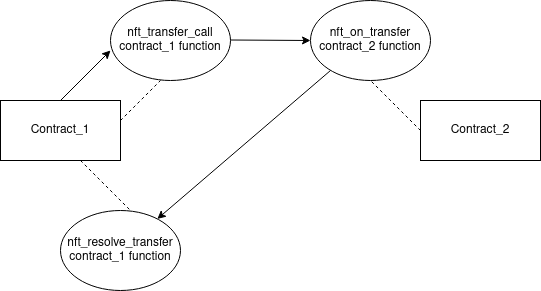
\includegraphics[height=70mm]{fig/temp.png}
	\caption{nft\_transfer\_call}
\end{figure}

Смоделируем пример, где мы хотим отправить из contract\_1 свой токен в другой контракт contract\_2 и выполнить в нем дополнительную сервисную логику(например contract\_2 это контракт маркетплейса, который должен будет выставить что-то на продажу).
Тогда сервисная логика должна будет реализована в nft\_on\_transfer. Вызывать ее должен будет nft\_transfer\_call и завершать всю эту цепочку должна будет функция nft\_resolve\_transfer.
Псевдокод функций будет выглядеть следующим образом:

\begin{listing}[H]
\begin{minted}[breaklines,fontsize=\scriptsize]{rust}
func nft_on_transfer(sender_id, previous_owner_id, token_id, msg) -> Promise;

#[payable]
fn nft_transfer_call(receiver_id, token_id, approval_id, msg) -> PromiseOrValue<bool> {

    /* Сохраняем отправителя и копию токена до отправки */
    sender_id = env::predecessor_account_id();
    previous_token = own_contract.internal_transfer(sender_id, receiver_id, token_id, approval_id);

    /* Если отправитель не владелец, значит мы ему доверили наш токен, подробнее в главе approval managements */
    authorized_id = None;
    if sender_id != previous_token.owner_id {
        authorized_id = sender_id;
    }

    /* Вызываем nft_on_transfer на другом контракте, потом nft_resolve_transfer на своем */
    reciever_contract::nft_on_transfer(
        sender_id,
        previous_token.owner_id,
        token_id,
        msg,
        receiver_id,
    ).then(
        own_contract::nft_resolve_transfer(
            authorized_id,
            previous_token.owner_id,
            receiver_id,
            token_id,
            previous_token.approved_account_ids,
        )
    )
}

#[private]
fn nft_resolve_transfer(
    authorized_id,
    owner_id, receiver_id,
    token_id, approved_account_ids,
) -> bool {

    /* Передача произошла успешно */
    if IsSuccesfull() {
        true
    }

    /* Иначе возвращаем токен обратно владельцу */
    own_contract.internal_remove_token_from_owner(receiver_id, token_id);
    own_contract.internal_add_token_to_owner(owner_id, token_id);
    token.owner_id = owner_id;
    refund_approved_account_ids(receiver_id, token.approved_account_ids);
    token.approved_account_ids = approved_account_ids;
    own_contract.tokens_by_id.insert(token_id, token);

    false
}
\end{minted}
\caption{NFT nft\_token}
\label{nftcontract.transfer}
\end{listing}

\paragraph{Enumeration}
Для удобного взаимодействия с контрактом, необходимо добавить больше view функций с pagination для просмотра NFT токенов\cite{enumstandard}:
\begin{enumerate}
\item nft\_total\_supply - получить общее количество существующих токенов.
\item nft\_tokens - получить существующие токены, используя pagination.
\item nft\_supply\_for\_owner - получить общее количество существующих токенов для конкретного аккаунта.
\item nft\_token\_for\_owner - получить существующие токены для конкретного аккаунта, используя pagination.
\end{enumerate}

Псевдокод будет выглядеть следующим образом:

\begin{minted}[breaklines,fontsize=\scriptsize]{rust}
pub fn nft_total_supply(&self) -> U128 {
    self.token_metadata_by_id.len()
}

pub fn nft_tokens(
    &self, from_index: Option<U128>,
    limit: Option<u64>
) -> Vec<JsonToken> {
    self.token_metadata_by_id.keys()
        .skip(from_index as usize)
        .take(limit.unwrap_or(15) as usize)
        .map(|token_id| self.nft_token(token_id.clone()).unwrap())
        .collect()
}

pub fn nft_supply_for_owner(
    &self,
    account_id: AccountId,
) -> U128 {
    if Exist(account_id) {
        self.tokens_per_owner.get(&account_id).len()
    } else {
        0
    }
}

pub fn nft_tokens_for_owner(
    &self,
    account_id: AccountId,
    from_index: Option<U128>,
    limit: Option<u64>,
) -> Vec<JsonToken> {
    if Exist(account_id) {
        tokens.iter()
            .skip(from_index as usize)
            .take(limit.unwrap_or(15) as usize)
            .map(|token_id| self.nft_token(token_id.clone()).unwrap())
            .collect()
    } else {
        return vec![];
    }
}
\end{minted}

\paragraph{Approval Management}
Необходимо добавить функционал передачи своего токена другим аккаунтом от своего имени\cite{approvalstandard}. Для этого будет хранить список доверенных аккаунтов(approved\_account\_ids).
Также структура токена хранит next\_approval\_id, который изначально равен 0 и увеличивается на единицу при каждом новом добавленном доверенном аккаунте.

Рассмотрим пример, где account\_1 решил создать токен, тогда у него будет следующая структура:
\begin{minted}[breaklines,fontsize=\scriptsize]{rust}
Token: {
    owner_id: account_1
    approved_accounts_ids: {}
    next_approval_id: 0
}
\end{minted}

Если он решит добавить account\_2, account\_3, как доверенные тогда структура станет следующей:
\begin{minted}[breaklines,fontsize=\scriptsize]{rust}
Token: {
    owner_id: account_1
    approved_accounts_ids: {
        account_2: 0,
        account_3: 1
    }
    next_approval_id: 2
}
\end{minted}

Счетчик next\_approval\_id  необходим, чтобы не случилось случая, когда новый владелец токена решил добавить доверенный аккаунт, который был до этого. Такие случаи могу испортить всю логику на других smart-контрактах.
Подробнее такие краивые случаи описаны в стандарте\cite{approvalstandard}.

Approval Management не добавляет новых внешних view функций или payable функций, а просто вносит некоторую дополнительную логику проверки в существующие функции из секции Core Functionality.

\paragraph{Royalties}

Последнее чего требует стандарт - распределение прибыли от продажи NFT или от любой другой логики, которая будет возвращать NEAR среди нескольких аккаунтов в зависимости от долей\cite{royaltystandard}.
Для этого у нас есть поле royalty в структуре Token, которая отображет пары в соответствующие доли. Сумма всех долей должна быть равна 10.000.

Также добавятся две новые функции:
\begin{enumerate}
\item nft\_payout - получить распределение баланса в зависимости от долей для конкретного token\_id.
\item nft\_transfer\_payout - совершить перевод токена и вернуть распределение баланса от долей.
\end{enumerate}
Псевдокод будет выглядеть следующим образом:
\begin{minted}[breaklines,fontsize=\scriptsize]{rust}
fn nft_payout(&self, token_id: TokenId, balance: u128, max_len_payout: u32) -> Payout {
    /* Проверить, что токен существует */
    assert(ExistToken(token_id))

    /* Достать структу токен */
    let token = self.tokens_by_id.get(&token_id);
    let mut current_sum = 0;
    let mut res = Payout {
        payout: HashMap::new()
    };

    /* Посчитать доли других аккаунтов */
    for (k, v) in token.royalty.iter() {
        let key = k.clone();
        if key == token.owner_id {
            continue;
        }
        res.payout.insert(
            key,
            calc_payout(*v, balance)
        );
        current_sum += *v;
    }
    /* Посчитать свою долю */
    res.payout.insert(
        token.owner_id,
        calc_payout(10000 - current_sum, balance)
    );
    res
}

#[payable]
fn nft_transfer_payout(
    &mut self,
    receiver_id: AccountId,
    token_id: TokenId,
    approval_id: u64,
    memo: Option<String>,
    balance: u128,
    max_len_payout: u32,
) -> Payout {
    /* Отправить токен */
    let sender_id = env::predecessor_account_id();
    let prev_token = self.internal_transfer(sender_id, receiver_id, token_id, approval_id, memo);

    let mut current_sum = 0;
    let mut result = Payout {
      payout: HashMap::new()
    };

    /* Посчитать доли других аккаунтов */
    for (k, v) in prev_token.royalty.iter() {
        let key = k.clone();
        if key == prev_token.owner_id {
            continue;
        }
        result.payout.insert(key, calc_payout(*v, balance));
        current_sum += *v;
    }
    /* Посчитать свою долю */
    result.payout.insert(prev_token.owner_id, calc_payout(10000 - current_sum, balance));
    result
}
\end{minted}

% \paragraph{Хранение содержимого}

% Стоит описать подход к хранению самого содержимого NFT, ведь в описанном стандарте в классе TokenMetadata у нас есть поле media,
% которое хранит в себе ссылку url на то, что из себя представляет NFT(картинка, аудио дорожка и так далее). В стандарте для хранения содержимого советуют использовать
% децентрализованное контентно-адресуемое хранилище. Примером такого хранилища может быть filecoin.io, который работает по протоколу Proof of Replication(PoRep)\cite{DBLP:journals/corr/abs-2002-10018}.
% В качестве хранилища было решено использовать Web3.storage~\cite{web3storage}. Они предоставляют удобное HTTP API и библиотеки на Go, Javascript для взаимодействия с хранилищем.

% Взаимодействие и логика связанная с загрузкой и выгрузкой содержимого в хранилище реализована на стороне Discord бота. За более подробным описанием можно обратиться к тексту сокомандника Ивана Луща.

\subsection{Структура маркетплейс smart-контракта}

В данной главе будет описано строение маркетплейс smart-контракта. Контракт маркетплейса уже не подчиняется никакому стандарту и может быть реализован разными способами.

\paragraph{Core functionality}

Начнем с функций, которые должны быть доступны пользователю:
\begin{enumerate}
    \item Выставить NFT токен на продажу.
    \item Обновить цену своего выставленного на продажу NFT токена.
    \item Убрать с продажи свой выставленный до этого NFT токен.
    \item Получить список выставленных на продажу NFT токенов.
    \item Купить выставленный на продажу NFT токен.
\end{enumerate}

Заметим, что на маркетплейс должны уметь выставлять токены нескольких NFT контрактов, потому что все они стандартизированны.
То есть пользователи могут покупать/продавать токены абсолютно разных NFT контрактов.

\begin{figure}[h!]
	\centering
	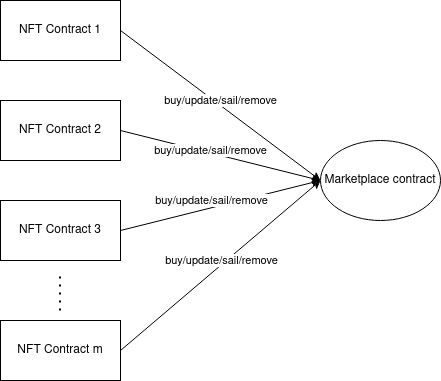
\includegraphics[height=70mm]{fig/marketplace.png}
	\caption{Marketplace core functionality}
\end{figure}

Опишем структуру маркетплейс контракта:

\begin{minted}[breaklines,fontsize=\scriptsize]{rust}

/* Так как выставить токен могут с разных контрактов, удобно будет соединить их в одной строке */
/* ContractAndTokenId = contract ID + DELIMITER + token ID */
pub type ContractAndTokenId = String;

/* Цена токенов будет в YoctoNear */
pub type SalePriceInYoctoNear = U128;

pub type TokenId = String;

/* Структура NFT токена выставленного на продажу */
#[derive(BorshDeserialize, BorshSerialize, Serialize, Deserialize)]
#[serde(crate = "near_sdk::serde")]
pub struct Sale {
    /* Владелец NFT токена */
    pub owner_id: AccountId,

    /* Значение этого поля обоснован в главе Approval Management */
    pub approval_id: u64,

    /* nft_contract_id с которого был выставлен NFT токен */
    pub nft_contract_id: String,

    /* Идендификатор выставленного токена */
    pub token_id: String,

    /* Цена */
    pub sale_conditions: SalePriceInYoctoNear,
}

/* Структура контракта */
#[near_bindgen]
#[derive(BorshDeserialize, BorshSerialize, PanicOnDefault)]
pub struct Contract {
    /* Владелец контракта */
    pub owner_id: AccountId,

    /* Выставленные на продажу токены по ContractAndTokenId */
    pub sales: UnorderedMap<ContractAndTokenId, Sale>,

    /* Выставленные на продажу ContractAndTokenId по конкретному аккаунту */
    pub by_owner_id: LookupMap<AccountId, UnorderedSet<ContractAndTokenId>>,

    /* Выставленные на продажу токены по конкретному аккаунту */
    pub by_nft_contract_id: LookupMap<AccountId, UnorderedSet<TokenId>>,

    /* Внесенная сумма на хранение nft токена */
    /* Смысл данной структуры будет обоснован позже */
    pub storage_deposits: LookupMap<AccountId, Balance>,
}
\end{minted}

Когда пользователь хочет выставить на продажу NFT токен, он должен вызвать nft\_approve у своего NFT контракта, чтобы добавить аккаунт маркетплейса в доверенные аккаунты, тогда на контракте маркетплейса вызовется метод nft\_on\_approve, который добавит токен на продажу.
В результате, когда другой пользователь захочет купить токен, то маркетплейс сможет легко перевести его новому владельцу, потому он является доверенным аккаунтом для продаваемого токена.

На иллюстрации будет приведен пример, где пользователь выставляет на продажу два токена с двух разных NFT контрактов на одном маркетплейс контракте.

\begin{figure}[H]
	\centering
	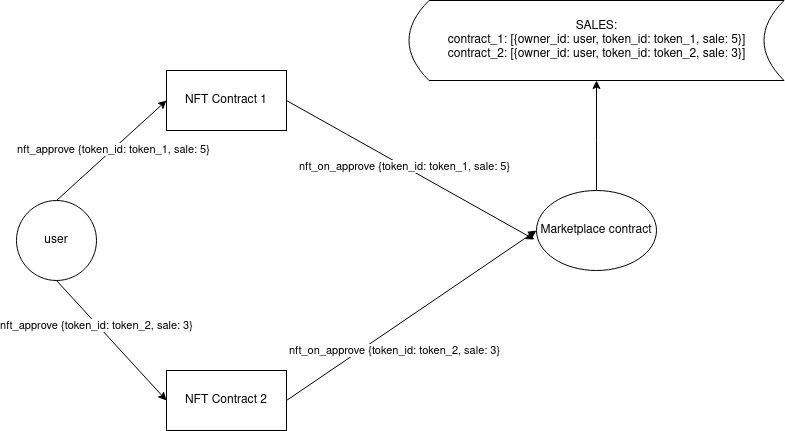
\includegraphics[height=70mm]{fig/sell.png}
	\caption{Marketplace contract sell}
\end{figure}

Псевдокод будет выглядеть следующим образом:

\begin{minted}[breaklines,fontsize=\scriptsize]{rust}
fn nft_on_approve(
    &mut self,
    token_id: TokenId,
    owner_id: AccountId,
    approval_id: u64,
    msg: String,
) {
    /* NFT контракт с которого был вызвана продажа */
    let nft_contract_id: AccountId = env::predecessor_account_id();

    /* Аккаунт пользователя, который подписал контракт */
    let signer_id: AccountId = env::signer_account_id();

    assert(owner_id == signer_id)

    /* Считаем сколько нужно на хранилище и сколько внесено */
    let paid_storage: u128 = self.storage_deposits.getPaidStorage(signer_id);
    let required_storage: u128 = CalcRequiredStorage();

    /* Проверяем, что денег на хранение достаточно */
    assert(paid_storage > required_storage);

    /* Sale conditions take from msg filed, if user don't fill msg it will panic */
    let sale_price  = GetSalePrice(msg);

    /* Добавляем покупку в необходимые структуры */
    let contract_and_token_id: String = nft_contract_id + '.' + token_id;
    self.sales.InsertNewSale(
        contract_and_token_id, owner_id, approval_id, nft_contract_id, token_id, sale_price
    );

    self.by_owner_id.InsertNewSale(
        contract_and_token_id, owner_id, approval_id, nft_contract_id, token_id, sale_price
    );

    self.by_nft_contract_id.InsertNewSale(
        owner_id, approval_id, nft_contract_id, token_id, sale_price
    );
}
\end{minted}

Так как мы делаем cross-contract call между двумя контрактами, тогда определить необходимые средства на хранения продаваемого NFT токена выглядит проблематичным.
Поэтому пользователь должен будет сам покупать хранилище и сам его освобождать, когда его токены продались и место освободилось. Именно для этого необходимо поле storage\_deposits в контракте.
Чтобы внести near под хранение используется функция storage\_deposit, а для вывода near за неиспользуемое место storage\_withdraw. Логика их кажется тривиальной, поэтому псевдокод приводиться не будет.

Изменение цены и отмена продажи, тоже выглядят достаточно тривиальными, напишем короткий псевдокод:

\begin{minted}[breaklines,fontsize=\scriptsize]{rust}
#[payable]
pub fn remove_sale(&mut self, nft_contract_id: AccountId, token_id: String) {
    /* Проверим, что владелец токена пытается его убрать с продажи */
    assert (self.sales.OwnerByToken(token_id) == env::precessor_account_id());

    /* Удаляем продажу из структур контракта */
    contract_and_token_id = nft_contract_id + '.' + token_id;
    self.sales.RemoveByToken(token_id);
    self.by_owner_id.RemoveByContractAndToken(owner_id, contract_and_token_id);
    self.by_nft_contract_id.RemoveByContractAndToken(contract_and_token_id, token_id);
}

#[payable]
pub fn update_price(
    &mut self,
    nft_contract_id: AccountId,
    token_id: String,
    price: U128,
) {
    /* Проверим, что владелец токена пытается его убрать с продажи */
    assert (self.sales.OwnerByToken(token_id) == env::precessor_account_id());

    /* Обновим цену продажы в структурах контракта */
    contract_and_token_id = nft_contract_id + '.' + token_id;
    self.sales.UpdateByToken(token_id, price);
}
\end{minted}

Последний пункт это покупка NFT токена.

\paragraph{Enumeration}

Для того, чтобы удобно взаимодействовать с маркетплейс контрактом были добавлены несколько view функций, которые позволяют выгружать продаваемые NFT.
\begin{enumerate}
\item get\_supply\_sales - получить суммарное количество выставленных токенов.
\item get\_supply\_by\_owner\_id - получить суммарное количество выставленных токенов за определенным пользователем.
\item get\_supply\_by\_nft\_contract\_id - получить суммарное количество выставленных токенов за определенным NFT контрактом.
\item get\_sales\_by\_nft\_contract\_id - получить выставленные на продажу токены за определенным NFT контрактом, используя pagination.
\item get\_sales\_by\_owner\_id - получить выставленные на продажу токены за определенным пользователем, используя pagination.
\item get\_sale - получить определенный продаваемый токен.
\end{enumerate}

Псевдокод данных функций будет выглядеть следующим образом:

\begin{minted}[breaklines,fontsize=\scriptsize]{rust}
pub fn get_supply_sales(
    &self,
) -> u64 {
    self.sales.len()
}

pub fn get_supply_by_owner_id(
    &self,
    account_id: AccountId,
) -> u64 {
    let owner_id = self.by_owner_id.get(&account_id);

    if let Some(owner_id) = owner_id {
        owner_id.len()
    } else {
        0
    }
}

pub fn get_sales_by_owner_id(
    &self,
    account_id: AccountId,
    from_index: Option<u128>,
    limit: Option<u64>,
) -> Vec<Sale> {
    let owner_id = self.by_owner_id.get(&account_id);

    let sales = if let Some(owner_id) = owner_id {
        owner_id
    } else {
        return vec![];
    };

    sales.iter()
        .skip(from_index)
        .take(limit)
        .map(|token_id| self.sales.get(&token_id).unwrap())
        .collect()
}

pub fn get_supply_by_nft_contract_id(
    &self,
    nft_contract_id: AccountId,
) -> u64 {
    let nft_contract_id = self.by_nft_contract_id.get(&nft_contract_id);

    if let Some(nft_contract_id) = nft_contract_id {
        nft_contract_id.len()
    } else {
        0
    }
}

pub fn get_sales_by_nft_contract_id(
    &self,
    nft_contract_id: AccountId,
    from_index: Option<u128>,
    limit: Option<u64>,
) -> Vec<Sale> {
    let by_nft_contract_id = self.by_nft_contract_id.get(&nft_contract_id);

    let sales = if let Some(by_nft_contract_id) = by_nft_contract_id {
        by_nft_contract_id
    } else {
        return vec![];
    };

    sales.iter()
        .skip(from_index)
        .take(limit)
        .map(|token_id| self.sales.get(&format!("{}{}{}", nft_contract_id, '.', token_id)).unwrap())
        .collect()
}

pub fn get_sale(&self, nft_contract_token: ContractAndTokenId) -> Option<Sale> {
    self.sales.get(&nft_contract_token)
}
\end{minted}

\section{Discord-бот}
\label{section.main.bot}

\subsection{Взаимодействие с блокчейнами}

В данной главе описано ядровое устройство discord-бота: описание работы near-api-js и его переписывание под устройство Discord, устройство метаданных NFT-токена, работа с децентрализованным распределенным хранилищем.

\paragraph{Аккаунты и access keys в NEAR}
Для понимания взаимодействия требуются минимальные знания об аккаунтах и access keys.

Аккаунты в NEAR\cite{nearaccounts} устроены так, что они имеют человеко-читаемый ID в отличие от большинства других блокчейнов, где обычно используется некоторый hash(Рисунок {\color{blue} \ref{fig.eth_near_cmp}}). Длина логина от 2 до 64 символов и содержит в конце суффикс обозначающий сеть блокчейна. Аккаунт может создавать подаккаунты, которые по своему функционалу ничем не отличаются от обычного аккаунта. Данные подаккаунты решают проблему деплоя контрактов: на один аккаунт можно развернуть только один smart-контракт, id аккаунта и будет значить, какой smart-контракт требуется.

\begin{definition}
    В NEAR, как и во всех блокчейнах есть несколько сетей: mainnet, testnet и так далее. Mainnet - главная(продакшн) сеть. Testnet используется для тестирования сервисов.
\end{definition}

Каждый аккаунт имеет создавать множество, которые в NEAR называются access keys. Существует два типа access keys: FullAccess и FunctionCall. Первый дает полный доступ, второй вид ключа уникален и дает разрешения только на подписание функций контрактов. В нашем сервисе не будет использоваться FullAccess access key из-за ненадобности.

\begin{figure}
    \centering
    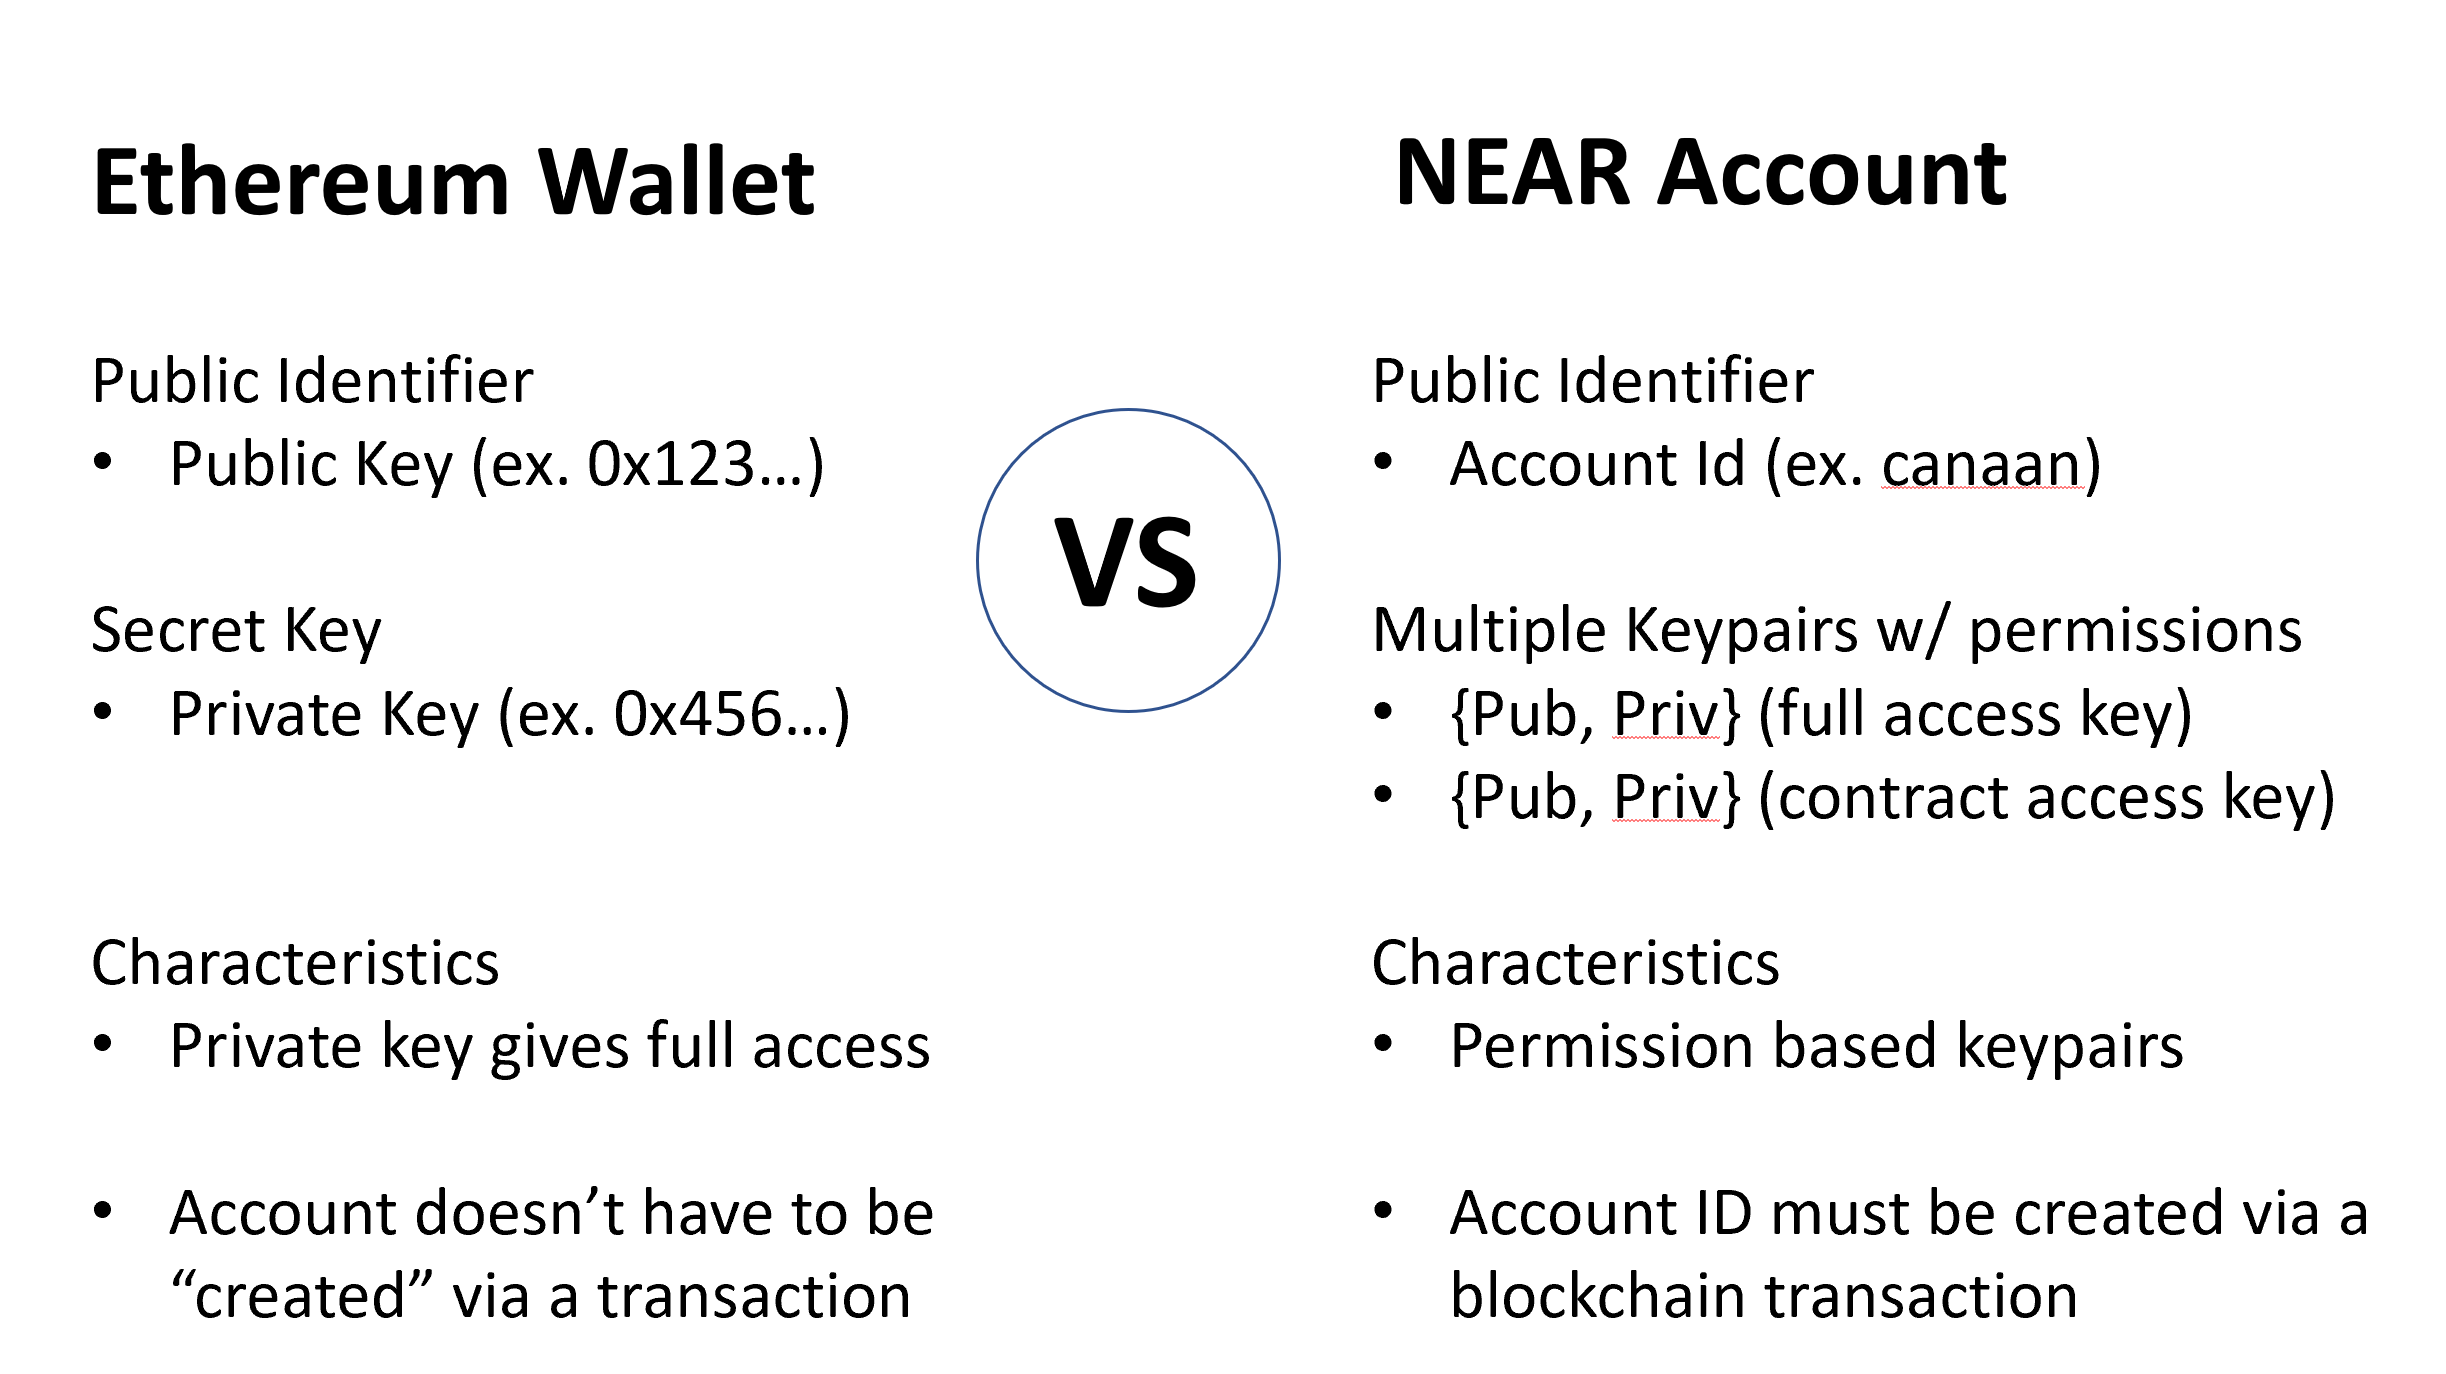
\includegraphics[height=60mm]{fig/eth_near_cmp.png}
    \caption{Сравнение аккаунтов Ethereum и NEAR}
    \label{fig.eth_near_cmp}
\end{figure}

\paragraph{Авторизация в NEAR Wallet}

Авторизация в NEAR Wallet играет роль связывания аккаунта кошелька и пользователя, то есть фактически нам говорит, что у этого пользователя есть этот аккаунт. Наверное, стоит отметить, что, если пользователь авторизовался в NEAR Wallet в нашем сервисе, то от его лица можно вызывать методы контракта, на котором была подписана транзакция(пока не закончатся GAS, которые были указаны при подписании транзакции), к которым не нужно вложение депозита. Данный функционал нам не потребуется, так как у нас либо <<view operations>> в контрактах, либо <<payable change operations>>.

На маркетплейсах в виде сайта вся авторизация происходит на client-side стороне: создается пара ключей(access key) - публичный и секретный; секретный ключ сохраняется в local storage браузера; подписывается транзакция и в последствии этот ключ будет использован сайтом, для подтверждения авторизации(Рисунок {\color{blue} \ref{fig.nearauth.a}}). Сценарий авторизации в discord-бот различается, ведь ключ должен храниться на стороне сервера(Рисунок {\color{blue} \ref{fig.nearauth.b}}). Для этого были необходимо реализовать KeyStore, который взаимодействует с какой-нибудь базой данных на стороне сервера. На роль БД было принято использовать Redis. Был написан KeyStore, который взаимодействует с Redis и функционал, который возвращает URL, а не редеректит пользователя. При любом взаимодействии с ботом, проверяется авторизован ли пользователь, если он не авторизован, то ему предлагается кнопка с URL на подписание транзакции авторизации.

\begin{figure}
	\centering
    \subfloat[Авторизация в NEAR Wallet в near-api-js]{
        \label{fig.nearauth.a}
        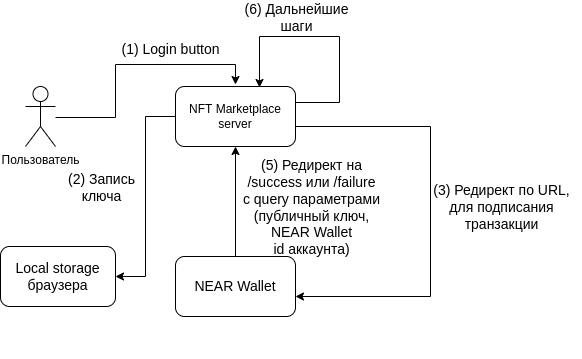
\includegraphics[height=60mm]{fig/auth1.png}
    }
    \subfloat[Авторизация в NEAR Wallet в discord-боте]{
        \label{fig.nearauth.b}
        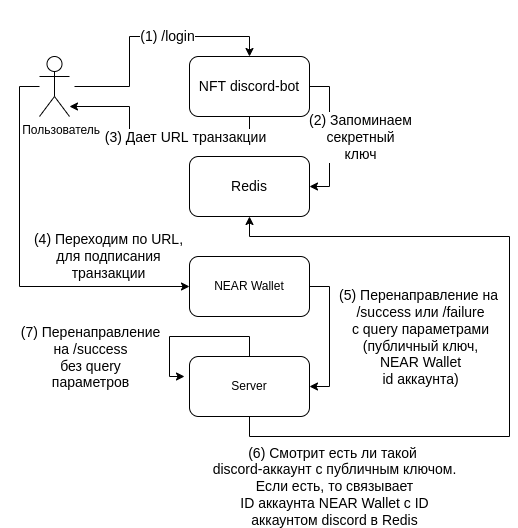
\includegraphics[height=80mm]{fig/auth2.png}
    }
    \caption{}
\end{figure}

\begin{definition}
    Storage --- интерфейс веб API, который позволяет добавлять, изменять, удалять элементы данных, которые представляются в виде ключа и значения\cite{webapistorage}. В веб API есть два объекта, которые используют интерфейс storage: session storage, local storage\cite{webapilocalstorage}. Session storage хранит данные до закрытия браузера, когда как данные в local storage не имеют ограничения по времени и могу быть удалены только намерено.
\end{definition}

\begin{definition}
    KeyStore\cite{nearclasskeystore} --- это класс, который хранит ключи, для подписей транзакций. Их 4 вида: BrowserLocalStorageKeyStore, InMemoryKeyStore, MergeKeyStore, UnencryptedFileSystemKeyStore. BrowserLocalStorageKeyStore пользуется локальным хранилищем браузера для записи, изменения, просмотра значений по ключу. InMemoryKeyStore хранит все в оперативной памяти, используется для тестирования. MergeKeyStore используется для объединения множества KeyStore. UnencryptedFileSystemKeyStore хранит все на диске в виде JSON файла, используется в near cli\cite{nearcli}.
\end{definition}

\paragraph{Вызовы методов у контрактов}

Вызовы методов у smart-контрактов --- это то, чем бот занимается большую часть времени.

\paragraph{Структура получаемого NFT и его метаданных}
\label{section.main.bot.struct}
На данный момент, при создании NFT в структуре(Листинг {\color{blue}\ref{lst.nftstructure}}) используются следующие поля: <<token\_id>>, <<owner\_id>>, <<royalty>>, <<metadata.title>>, <<metadata.media>>, <<metadata.reference>>. <<metadata.description>> не используется, все описание NFT хранится в метаданных в децентрализованном хранилище в целях экономии оплаты за хранение . В <<metadata.media>>, <<metadata.reference>> хранятся полные URL до медиа-файла и метаданных. В ближайшее время, планируется хранить только CID и только в поле media, так как медиа-файл и метаданные хранятся в одной директории, то для их определения достаточно одного CID(см. {\color{blue} \ref{section.main.bot.storage}}).

Структура метаданных(Листинг {\color{blue}\ref{lst.nftmetadata}}) полностью аналогично структуре метаданных в Paras, так как эта структура оправдана своей функциональностью. Только в отличие от Paras нет полей: <<collection>>, <<collection\_id>>, <<blurhash>>, <<mime\_type>>. <<collection>>, <<collection\_id>> нет, потому что на данный момент мы не поддерживаем коллекции NFT. <<mime\_type>>, <<blurhash>> из-за ненадобности.

\begin{listing}
\begin{minted}[breaklines,fontsize=\scriptsize]{js}
{
    token_id: 'chopik.testnet.1652636744470',
    owner_id: 'chopik.testnet',
    approved_account_ids: { 'papamsmarket.pojaleesh.testnet': 2 },
    royalty: { 'chopik.testnet': 10000 },
    metadata: {
        title: 'City',
        description: null,
        media: 'https://bafybeiahhurffoxjubs42l7bl3jjc5zk5vrafiijcxkhex2ukjm3zsbbti.ipfs.dweb.link/f',
        media_hash: null,
        copies: null,
        issued_at: null,
        expires_at: null,
        starts_at: null,
        updated_at: null,
        extra: null,
        reference: 'https://bafybeiahhurffoxjubs42l7bl3jjc5zk5vrafiijcxkhex2ukjm3zsbbti.ipfs.dweb.link/m',
        reference_hash: null
    }
}
\end{minted}
\caption{Структура получаемого NFT}
\label{lst.nftstructure}
\end{listing}

\begin{listing}
\begin{minted}[breaklines,fontsize=\scriptsize]{json}
{
    "description":"Cool city",
    "creator_id":"chopik.testnet",
    "attributes":[
        {"trait_type":"Time","value":"Night"},
        {"trait_type":"Color","value":"Blue"}
    ]
}
\end{minted}
\caption{Структура метаданных NFT в децентрализованном хранилище}
\label{lst.nftmetadata}
\end{listing}

\paragraph{Децентрализованное хранилище данных}
\label{section.main.bot.storage}

Обычно для хранения метаданных и медиа-объекта используется другой блокчейн специализированный под хранение. Связанно это с тем, что при деплое smart-контракта пользователь платит в NEAR за хранение байт, которые хранит контракт, используя механизм, который называется storage staking. На основе storage stacking есть и атаки на smart-контракты, например <<million cheap data additions>> - злоумышленник добавляет огромное количество бесполезных данных при вызове методов, из-за этого в наших контрактах данное обложение в контрактах оплачивает пользователь, которому хочется минимизировать свои растраты на операции. Из-за этого лучше стратегий для хранения объемных файлов(в основном таковыми являются медиа-файлы) это хранить данные в off-chain. Популярным решением является IPFS, при котором любой набор данных представляется удобным адресом - CID. В роли сервиса предоставляющего хранилище был выбран NFT.Storage\cite{nftstorage} --- бесплатное децентрализованное хранилище NFT на IPFS\cite{ipfs} и Filecoin\cite{filecoin}. NFT.Storage предоставляет HTTP API для взаимодействия с хранилищем и обертку на Javascript.

\begin{remark}
    Цена на storage staking устанавливается сетью блокчейна, на данный момент это 1 NEAR за 100 КБ.
\end{remark}

\begin{definition}
    IPFS(InterPlanetary File System) - это протокол распределенной системы обмена файлов. При добавлении файла в IPFS, он делится на маленькие куски, криптографически хэшируется и отдается уникальный фингерпринтр, который называется CID(Content identifier) \cite{ipfs}.
\end{definition}

\begin{remark}
    Для того, чтобы построить стимулирующий слой для сохранения данных в IPFS существует Filecoin. Filecoin - это децентрализованное сетевое хранилище. Filecoin и IPFS - это два разных протокола, взаимодополняющие друг друга. Когда как IPFS позволяет пользователям хранить, запрашивать и передавать друг другу данные, в то время, как Filecoin предназначен для обеспечения системы постоянного хранения.
\end{remark}

\begin{remark}
    Изначально использовался сервис web3storage\cite{web3storage} для хранения, но он отличился медленной загрузкой, получением файлов, из-за чего появилась необходимость в смене на NFT.Storage.
\end{remark}

\subsection{Пользовательский интерфейс}

\paragraph{Точки входа}

\begin{figure}
    \centering
    \subfloat[Slash-команды бота]{
        \label{fig.slashcommands}
        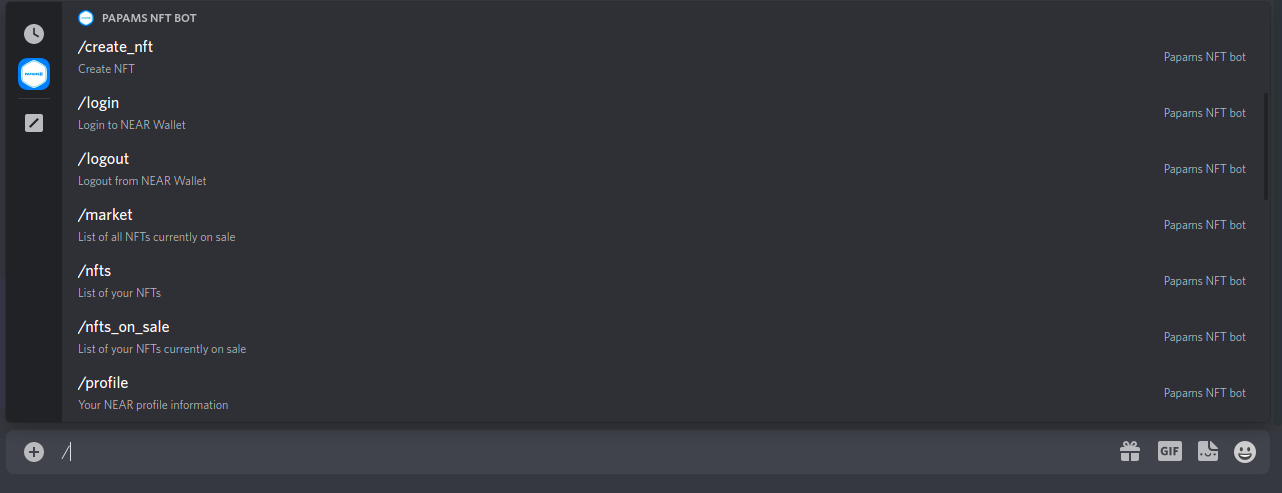
\includegraphics[height=60mm]{fig/slash_commands.png}
    }\\
    \subfloat[Контекстные меню бота]{
        \label{fig.contextmenu}
        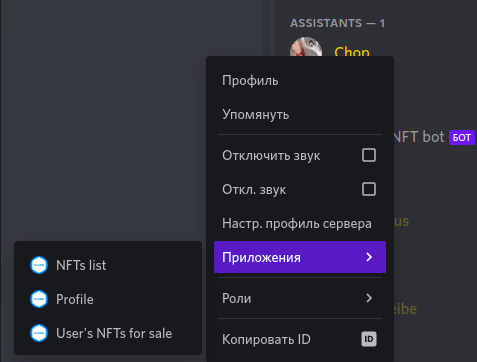
\includegraphics[height=70mm]{fig/context_menu.png}
    }
    \subfloat[Профиль пользователя]{
        \label{fig.profile}
        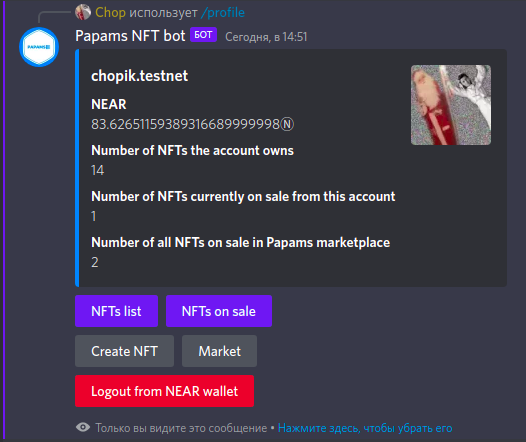
\includegraphics[height=70mm]{fig/profile.png}
    }
    \caption{Точки входа пользователя}
\end{figure}

\begin{figure}
    \centering
    \subfloat[Намереная авторизация]{
        \label{fig.authbtn1}
        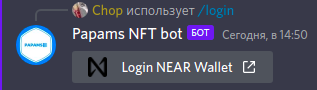
\includegraphics[height=30mm]{fig/authbtn1.png}
    }\\
    \subfloat[Предложение об авторизации]{
        \label{fig.authbtn2}
        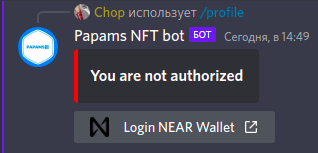
\includegraphics[height=30mm]{fig/authbtn2.png}
    }
    \caption{Авторизация пользователя}
\end{figure}

\begin{figure}
    \centering
    \subfloat[Slash-команды бота]{
        \label{fig.mynftlistonsale}
        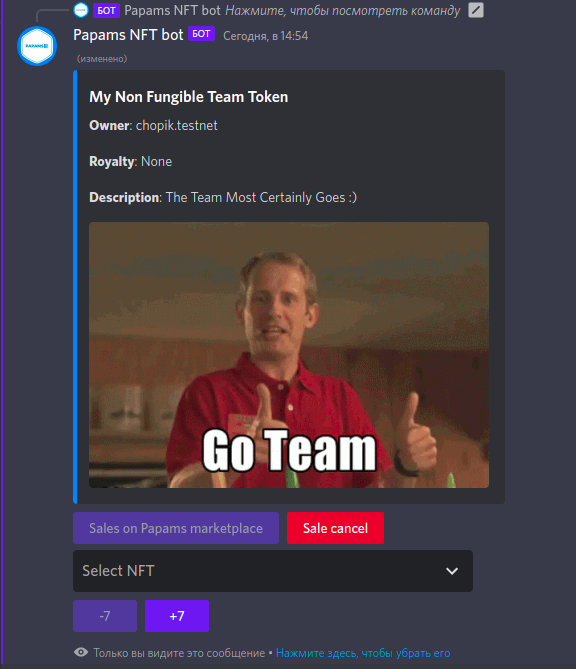
\includegraphics[height=70mm]{fig/mynftlistonsale.png}
    }
    \subfloat[Контекстные меню бота]{
        \label{fig.contextmenu}
        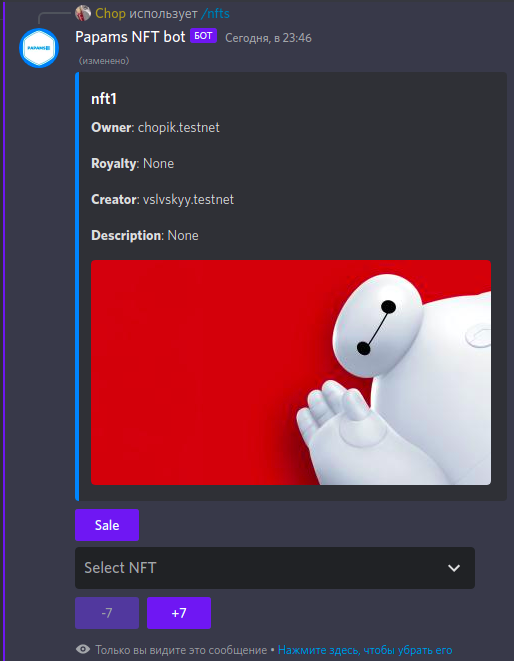
\includegraphics[height=70mm]{fig/mynftlistcansale.png}
    }\\
    \subfloat[Профиль пользователя]{
        \label{fig.profile}
        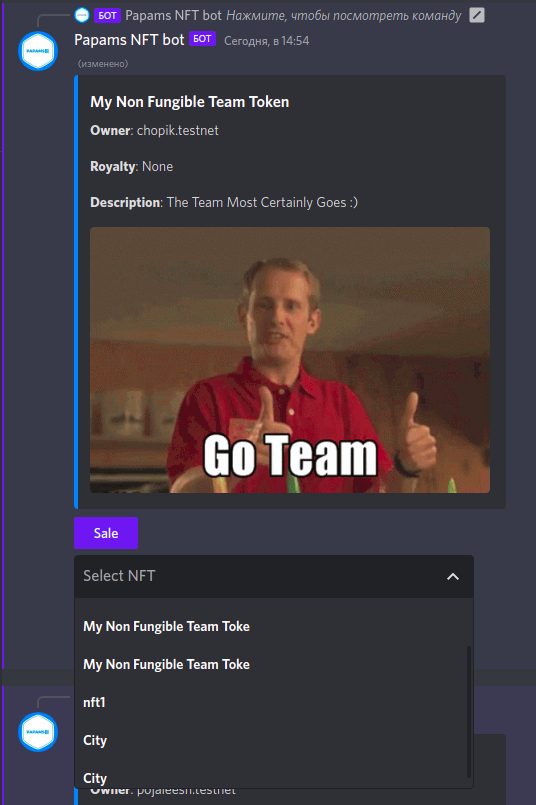
\includegraphics[height=80mm]{fig/mynftwidth.png}
    }
    \caption{Точки входа пользователя}
\end{figure}

\section{Генеративно-состязательная сеть}
\label{section.6}
// Текст будет написан Токкожиным Арсеном
\section{Сервис с генеративно-состязательной сетью}
// Текст будет написан Кусиденовым Адильханом

\label{section.7}
